\chapter{Mercoledì 04/03/2020}
\paragraph{Sistema organizzativo} Ogni azienda basa la propra esistenza su un sistema organizzativo, cioè un insieme di risorse e regole atte a perseguire in modo coordinato le esigenze della stessa. Con risorse intendiamo persone, denaro, materiale, ma soprattuto informazioni!  
\paragraph{Sistemi informativi} La componente del sistema organizzativo che si occupa di ogni singolo processo (aggiunta, manipolazione, ma anche conservazione...) che ha a che fare con l'informazione è detta \emph{sistema informativo}. Il mantenimento dell'informazione è vitale per ogni azienda ed ente! Il concetto è indipendente da qualsiasi forma di automatizzazione: i sistemi informativi esistono da secoli, ancora prima della nascita dell'informatica (le banche hanno sempre conservato moli elevate di informazioni fin dalla loro nascita).
\paragraph{Sistema informativo automatizzato} Oggi i sistemi informativi mantengono le informazioni mediante un approccio informatico (\emph{sistema informatico}): è inevitabile, soprattutto nelle grandi aziende, il ricorso a tecnologie informatiche.

\section{Base di dati}
Il cuore del sistema informativo automatizzato è la \emph{base di dati}, un insieme organizzato di dati da cui possiamo trarre le informazioni di nostro interesse.

\subsection{Differenza tra dati e informazioni}
\paragraph{Informazione} Una notizia, un dato o un elemento che permette di avere conoscenza di ciò che ci circonda. L'interpretazione dell'informazione, la \emph{decodifica}, ci porta al dato.
\paragraph{Dato} Il dato è un concetto generale, la rappresentazione simbolica di un qualunque tipo di informazione all'interno del sistema informatizzato. La codifica dell'informazione è parte sostanziale del progetto della base di dati: decideremo di rappresentare qualcosa mediante stringhe, qualcos'altro mediante interi... e così via.
\begin{itemize}
	\item I dati non hanno alcun significato da soli, ma se contestualizzati possono portarci a conoscere delle informazioni. Prendiamo una stringa \emph{Mario} e il numero 9. Individualmente non hanno alcun significato, ma in un certo contesto possono portarci a conoscere delle informazioni: il numero 9 all'anagrafe potrebbe essere l'età della persona, a scuola una valutazione didattica....
	\item I dati sono un qualcosa di tendenzialmente stabile nel tempo. Gli enti pubblici negli ultimi anni hanno adottato l'approccio informatico nella conservazione dell'informazione, adottando nuove proceure: queste hanno ereditato i dati già in possesso dei vari enti.
	\item I dati costituiscono un patrimonio significativo da sfruttare e proteggere. Basta pensare al grande potere di chi possiede dati: i governi, che possono tassarti; le agenzie di marketing, che possono sfruttare informazioni personali o la tua cronologia per suggerirti prodotti più interessanti; i social, i cui dati possono essere utilizzati da chiunque per poter conoscere le tendenze del momento... 
	
\end{itemize}
\subsection{Caratteristiche di una base di dati}
Le basi di dati sono
\begin{itemize}
	\item \textbf{grandi}: una base di dati possono contenere una mole elevatissima di dati. La dimensione di una base può essere superiore a quella della memoria centrale e raggiungere milioni di gigabyte. Un sistema deve essere in grado di gestire \emph{memorie secondarie}. Ovviamente una base di dati può essere anche piccola, ma i sistemi devono poter gestire una base indipendentemente dalla loro dimensione.
	\item \textbf{condivise}: la base di dati è una risorsa integrata e condivisa tra più settori di un'organizzazione, ciascuno con un proprio sottosistema informativo. Applicazioni e utenti diversi devono poter accedere a dati comuni: mediante un meccanismo di \emph{controllo di concorrenza} il sistema gestisce le operazioni svolte in contemporanea da più utenti. \\Una base di dati può essere utilizzata anche per scambiare informazioni: se un programma all'interno di questo "ecosistema" modifica i dati della base gli altri programmi visualizzeranno i dati aggiornati (effettivamente uno scambio).
	\item \textbf{persistenti}: le basi di dati non hanno un tempo di vita collegato all'esecuzione dei programmi che le utilizzano.
\end{itemize}
\subsection{Perchè utilizziamo una base di dati?}
L'approccio della base di dati ci permette di evitare ridondanze ed errori. Prendiamo un esempio: gli uffici amministrativi, fino a qualche anno fa, conservavano le informazioni in modo cartaceo. Ogni ufficio possedeva un "archivio cartaceo" caratterizzato da centinaia di documenti. Non esisteva, ovviamente, un sistema centralizzato.
\begin{itemize}
	\item L'ufficio anagrafe conserva i certificati di nascita
	\item L'ufficio che si occupa delle unioni civili conserva gli atti di matrimonio.
\end{itemize}
Senza un sistema centralizzato non si hanno controlli di consistenza: l'aggiornamento di uno dei due archivi non comporta automaticamente l'aggiornamento di informazioni simili contenute in altri. Presumiamo sia morto un certo \emph{Mario bianchi}: all'anagrafe risulta morto, ma al secondo ufficio risulta sposato a partire da una data successiva alla morte.
\section{Il \emph{DBMS}}
Adottando l'approccio della base di dati otteniamo un sistema integrato privo di ridondanze ed errori. Ciò risulta vantaggioso anche i termini di memoria: invece di avere più archivi contenenti le stesse informazioni ne abbiamo uno solo.
\paragraph{Università di Pisa} La nostra università è divisa in tanti dipartimenti e settori: ciascuno di essi può accedere a un vasto sistema informatico che copre tutto l'ateneo. Esso raccoglie i dati di ogni singolo studente e riduce la possibilità di ridondanze e incoerenze mediante una gestione centralizzata. Pensiamo al portale \emph{Valutami}: i voti dell'ateneo o le prenotazioni non sono gestite da ogni singolo dipartimento ma da un sistema utilizzato da ogni singola facoltà. Altro esempio potrebbero essere le mense: i dati da loro utilizzati (i soldi rimasti sulla carta, l'ISEE,\dots) sono prelevati dallo stesso sistema informatico!
\paragraph{Chi si occupa dei controlli di consistenza (fino ad ora non possibili)?} Il \emph{DBMS}!
\begin{definizione}[Base di dati - definizione informatica]
	Collezione di dati grandi, persistenti e condivisi gestita da un \emph{DBMS}
\end{definizione}
\begin{definizione}[\emph{DBMS}]
	Questa sigla è acronimo di \emph{Data Base Management System}. Esso è un sistema software in grado di gestire collezione di dati.
\end{definizione}
\subsection{Ruolo del \emph{DBMS}}
Il \emph{DBMS} "protegge" la base di dati e garantisce 
\begin{itemize}
	\item \textbf{affidabilità} (la cosa più importante): i dati, come già detto \emph{persistenti}, devono rimanere inalterati finchè non manipolati da un utente. Il sistema deve prevedere meccanismi di \emph{backup} e \emph{recovery} in caso di malfunzionamenti per non perdere definitivamente i dati salvati.
	\item \textbf{privatezza}: gli utenti devono avere accesso soltanto ai dati di cui hanno bisogno e possono eseguire soltanto le operazioni necessarie. Mediante un sistema di \emph{autorizzazioni} l'amministratore gestisce gli accessi degli utenti stabilendo le operazioni permesse.
	\item \textbf{efficienza}: devono svolgere operazioni in tempi accettabili per l'utente utilizzando al meglio le risorse di memoria a disposizione. I DBMS richiedono molte risorse per il numero elevato di funzionalità disponibili. L'efficienza può essere garantita solo con sistemi informatici adeguati accompagnati da investimenti.
	\item \textbf{efficacia}: devono rendere produttiva l'attività di ogni singolo utente. Il sistema deve essere adeguatamente dimensionato e la base ben progettata.
\end{itemize}
Ricordiamo la presenza di \emph{controlli di concorrenza} per garantire la possibilità di informazioni simultanee.
%\subsection{Ruolo del DBMS}
%Il DBMS, che possiamo chiamare anche gestore, "protegge" la base di dati: mantiene l'integrità della struttura in caso di problemi. Si occupa della base di dati e garantisce la sua consistenza nel corso di interrogazioni. Garantisce la possibilità di informazioni simultanee (\emph{controlli di concorrenza}). Gestisce le autenticazioni garantendo l'accesso degli utenti esclusivamente ai dati necessari limitando le operazioni possibili (\emph{sistema di autenticazioni}). 
\subsection{Dizionario dei dati, sistema operativo} Parte della base di dati contiene il cosiddetto \emph{dizionario dei dati}: una descrizione unica e centralizzata dei dati utilizzabile dai vari programmi. Il salvataggio dei dati avviene mediante file, ma le funzionalità del file system risultano estese e si hanno più servizi.
\begin{center}
	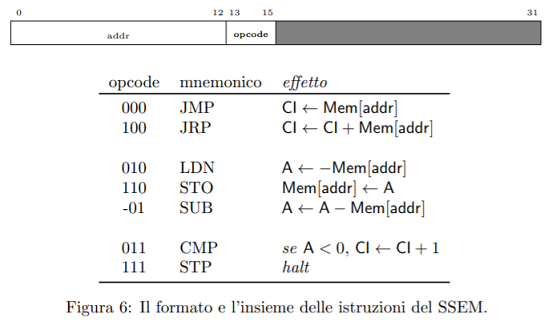
\includegraphics{images/1.png}
\end{center}
\subsection{Indipendenza dei dati} 
L'architettura scelta deve garantire l'\emph{indipendenza dei dati}. Questa consiste nella \underline{principale} proprietà del DBMS. Si permette a utenti e programmi applicativi che utilizzano una base di dati di interagire a un elevato livello di astrazione, che prescinde dai dettagli realizzativi utilizzati nella costruzione della base di dati. L'indipendenza dei dati si articola in
\begin{itemize}
	\item \textbf{indipendenza fisica}: si interagisce col DBMS in modo indipendente dalla struttura fisica dei dati. Posso modificare le strutture fisiche senza influire sulle descrizioni dei dati ad alto livello
	\item \textbf{indipendenza logica}: si interagisce col livello esterno della base in modo indipendente dal livello logico. Posso creare uno schema esterno in base a certe esigenze senza dover modificare lo schema logico. Inoltre, posso modificare il modello logico senza dover modificare le strutture esterne.
\end{itemize}
Fondamentalmente quanto detto rappresenta la differenza tra interfaccia e implementazione vista a \emph{Fondamenti di programmazione}.
\subsection{Vantaggi e svantaggi}
\subsubsection{Vantaggi}
\begin{itemize}
	\item Gestione centralizzata (e conseguente riduzione di ridondanze ed errori) con possibilità di “economia di scala”
	\item Disponibilità di servizi integrati per un'intera organizzazione (maggiore produttività)
	\item Indipendenza dei dati (favorisce lo sviluppo e la manutenzione delle applicazioni)
\end{itemize}
\subsubsection{Svantaggi} 
\begin{itemize}
	\item Costo dei prodotti e della transizione verso di essi
	\item Non scorporabilità (spesso) delle funzionalità (con riduzione di efficienza)
\end{itemize}
In certe circostanze può risultare utile, soprattutto quando lavoriamo in ambienti piccoli, ricorrere a un approccio più tradizionale nella conservazione dei dati.


\section{Concetto di \emph{transazione}}
Tutti i gestori attualmente in commercio sono detti \emph{transazionali} poichè basati su transazioni (forniscono meccanismi per definire ed eseguire transazioni).\\
La transazione consiste in un insieme di operazioni (di lettura e scrittura della memoria)
\begin{itemize}
	\item \textbf{indivisibili} (atomicità). Questo significa che se una delle operazioni non può essere eseguita allora la transazione nel suo complesso non può essere eseguita (Esempio: transazione bancaria, compio un prelievo da un conto A e un versamento in un conto B)
	\item \textbf{corrette} anche in presenza di concorrenza (controllo della concorrenza)
	\item \textbf{con effetti definitivi} (permanenza)
\end{itemize} Non possiamo vedere lo stato di questa sequenza, ma solo l'inizio e la fine: ciò che avviene nel mezzo non è detto sia corretto, l'importante è che al termine tutto sia effettivamente corretto.\\
Le transazioni possono essere molto complesse e in alcuni casi provocare errori: lo svolgimento di transazioni deve essere bloccato nel caso in cui possano emergere problemi. Il gestore, ogni volta, stabilisce se l'utente può effettivamente svolgere operazioni.\\
Quando la transazione termina con successo si ha un risultato di  tipo \emph{commit} (impegno) e quanto fatto viene salvato, altrimenti si ha un risultato di tipo \emph{aborted} (abortito) e non vengono apportate modifiche.
\section{Modello logico}
\paragraph{Perchè parliamo di modelli logici?} I programmi fanno riferimento ai dati, la cui struttura deve poter essere modificata senza modificare i programmi. Proprio per questo andiamo ad introdurre il \emph{modello logico}, un insieme di costrutti utilizzati per organizzare i dati. Un'organizzazione dei dati, distinta da quella dell'applicazione, permette di dividere l'interfaccia dall'implementazione con un approccio non diverso da quello visto con i moduli a \emph{Fondamenti}: il DBMS nasconde  l'implementazione e gli utenti si trovano in un livello astratto da cui possono compiere interrogazioni senza conoscere la struttura.
\paragraph{Esempio} Un esempio è il \emph{modello relazionale}, il cui costrutto caratterizzante è la relazione. Essa permette di definire insiemi di record omogeni a struttura fissa: una tabella.
\subsection{Schema e istanza}
Ogni tipo di dato nel modello logico è caratterizzato da
\begin{itemize}
	\item uno schema, sostanzialmente invariato nel tempo, che descrive la struttura
	\item un'istanza, i valori, che può variare rapidamente nel tempo.
\end{itemize}
Nel modello relazionale lo schema consiste nella prima riga della tabella, l'istanza nel corpo della stessa.
\section{Linguaggi per basi di dati}
Il linguaggio utilizzato permette la definizione degli schemi e la manipolazione delle tabelle. Si distinguono due tipi di linguaggio:
\begin{itemize}
	\item il \emph{Data definition language} (DDL) per la definizione di schemi
	\item il \emph{Data manipulation language} (DML) per l'interrogazione e l'aggiornamento
\end{itemize}
Alcuni linguaggi presentano entrambe le funzioni. Il più noto è l'SQL: è detto linguaggio testuale e interrattivo poichè un utente può scrivere l'interrogazione ed eseguirla immediatamente.
\subsection{Immersione in linguaggio ospite}
Caratteristica importante è la possibilità di "immergere" i comandi SQL in un linguaggio ospite: in Java, in C++, in PHP. Questo discorso è affrontato in un capitolo successivo.

\section{Architettura del DBMS}
Con architettura intendiamo il modello di esecuzione utilizzato da un sistema in cui esiste un DBMS. Tutte le realizzazioni di gestori utilizzano un'\emph{architettura distribuita}, caratterizzata dalla presenza di più macchine che lavorano autonomamente e interagiscono mediante la rete.
\subsection{Architettura a due livelli - \emph{client-server}}
L'architettura più diffusa è quella \emph{client-server}, detta anche \emph{a due livelli}. Abbiamo due macchine che comunicano attraverso la rete:
\begin{itemize}
	\item il server. Ha la base di dati e il DBMS, offre servizi e risponde alle richieste dei client.
	\item il client. Richiede servizi comunicando con il server attraverso la rete.
\end{itemize}
In alcune circostanze la macchina potrebbe fungere sia da server che da client, normalmente ciò non avviene. Il server deve avere la potenza sufficiente per svolgere tutte le operazioni richieste dai client in tempi accettabili. Ovviamente possono esserci più server e avere una base di dati distribuita.\\
Individuiamo due tipi di client:
\begin{itemize}
	\item \textbf{thin client} (il più diffuso): l'elaborazione dei dati (\emph{logica dell'applicazione}) avviene nel server. 
	\item \textbf{thick client}: l'elaborazione dei dati avviene nel client. Ciò può risultare svantaggioso: la macchina deve essere potente per trasmettere i dati a tutti i client e ognuna deve avere un rapporto fiduciario col gestore di dati. Inoltre non si possono avere più di poche centinaia di client.
\end{itemize}
\subsection{Architettura a tre livelli}
Con internet si passa a un'architettura \emph{a tre livelli}. Essa presenta:
\begin{itemize}
	\item un server contenente la base di dati
	\item un server applicativo che compie elaborazioni
	\item un client che compie interrogazioni
\end{itemize}
Anche in questo caso si possono avere più server, sia del primo tipo che del secondo. Il client, invia le richieste al server applicativo e questo dialoga con il server contenente la base di dati. 
\paragraph{Quale vantaggio si cela dietro questa struttura?} Il client è di tipo \emph{thin} e si occupa esclusivamente dell'interfacciamento (quindi possibile numero di client maggiore). In un certo senso il client coincide con il browser web! 
\paragraph{Sistemi eterogenei} Possiamo connettere sistemi non omogenei: posso compiere le solite domande che sono abituato a fare senza rendermi conto, per esempio, di avere un database di diverso tipo.
\section{Big Data}
Per definizione gli oggetti contenuti in base di dati sono di dimensioni enormi. Nel tempo abbiamo visto l'introduzione di strumenti informatici sempre più evoluti e l'aumento di produzione di dati. Descriviamo la cosa mediante le quattro v:
\begin{itemize}
	\item \textbf{Volume}: in un minuto si ottiene già una grande quantità di dati. Milioni di interrogazioni a Google, di like e share su Facebook, di downloads da youtube... 
	\item \textbf{Velocità}: i dati si muovono ad alta vellocità. Esistono tecniche che permettono di analizzare i flussi: non salvo i dati ma i risultati dell'analisi dei flussi.
	\item \textbf{Varietà}: i dati non sono più esclusivamente strutturati in tabella, ma prevalentemente non strutturati (testi, immagini, vocali, video)
	\item \textbf{Veridicità}: i dati estratti sono veritieri? Posso estrarre informazioni vere anche in presenza di gravi errori, imprecisioni e incompletezze. 
\end{itemize}
\paragraph{\emph{data science}} La qualità deve essere sempre garantita: ciò ha favorito la nascita della \emph{data science}, una branca dell'informatica che collabora con la matematica (in particolare con la statistica). La data science include i seguenti aspetti:
\begin{itemize}
	\item \emph{Data cleaning}: costruzione di una raccolta dati con un sufficiente livello di qualità
	\item \emph{Data integration}: costruzione di una raccolta dati integrata a partire da differenti sorgenti.
	\item \emph{Data mining}: estrazione di informazioni utili dai dati.
	\item \emph{Metodi predittivi} Metodi per prevedere mediante osservazioni nel passato dati riguardanti il futuro
	\item \emph{Machine learning}: metodo predittivo particolare. Vengono forniti alla macchina dei dati iniziali, che ne permettono l'educazione e una progressiva autonomia nell'analisi dei dati.
\end{itemize}
\paragraph{\emph{Data engineers}} Noi ingegneri ci occuperemo soprattutto delle infrastrutture per analizzare i dati (e non delle tecniche di analisi come il \emph{data scientist}).

\section{Sistemi non relazionali e potenziamento di un sistema} Negli ultimi anni sono emersi nuovi sistemi non relazionali in cui si rinuncia ad alcuni elementi citati fino ad ora per ottenere maggiore flessibilità. I sistemi NoSQL, per esempio, non hanno una vera e propria struttura dati: semplicemente mi limito ad aggiungere e rimuovere colonne quando necessario. Sia i dati che gli utenti tendono ad aumentare e quindi risulta necessario scalare. Posso adottare uno dei seguenti approcci:
\begin{itemize}
	\item scalare verticalmente, quindi adottare un approccio centralizzato e aumentare la potenza dei miei server (costi elevati)
	\item scalare orizzontalmente, approccio distribuito in cui posso aggiungere nuovi server standard e non potentissimi (economico)
\end{itemize} 
L'ultimo approccio è quello adottato con i database \emph{NoSQL}. Ho Mario Bianchi: ogni volta che ho informazioni nuove su di lui continuo ad aggiungerle. Ottengo delle liste. Questi sistemi sono utili in particolare quando abbiamo una crescita molto elevata, quasi incontrollata, di dati. La loro semplicità, tuttavia, è dovuta anche alla mancanza di controlli sull'integrità dei dati: il compito ricade sull'applicazione che dialoga col database.  Inoltre l'assenza di una vera e propria struttura dati rende difficile il passaggio a un altro tipo di database. Segue che questi database non domineranno mai il mercato.
\pagebreak

\section{Modello relazionale}
Il \emph{modello relazionale} si basa sul concetto matematico di relazione, con alcune differenze. Esso permette di definire insiemi di record omogeni a struttura fissa: una tabella.
\paragraph{Prodotto cartesiano}
Dati $n$ insiemi $D_1,\dots,D_n$ (che costituiscono i domini del prodotto cartesiano) non necessariamente distinti il prodotto cartesiano $D_1 \times \dots \times D_n$ consiste nell'insieme delle \emph{n-uple} ordinate $(v_1,\dots,v_n)$ dove $v_k \in D_k, k=1\dots n$. Il prodotto cartesiano può essere svolto anche tra insiemi che non presentano la stessa cardinalità.
\paragraph{Relazione matematica}
Una relazione matematica sugli insiemi $D_1,\dots,D_n$ consiste in un sottoinsieme del prodotto cartesiano $D_1 \times \dots \times D_n$ (quindi si considerano solo parte delle \emph{n-uple ordinate} effettivamente ottenute col prodotto cartesiano)
\paragraph{Grado del prodotto cartesiano}
Il grado del prodotto cartesiano consiste nel numero delle componenti di ogni \emph{n-upla} del prodotto cartesiano.
\paragraph{Cardinalità della relazione}
La cardinalità della relazione consiste nel numero delle \emph{n-uple} ottenute.

\noindent Si ha (nella matematica) una \emph{struttura posizionale} in cui la posizione consiste nell'indice del dominio. Si individua il ruolo di ciascun dominio a partire dalla posizione. L'ordine delle colonne ha un significato ben preciso, mentre l'ordine delle righe non ha importanza (non essendo numerate non si hanno n-uple, ma tuple).
\subsection{Passaggio a struttura non posizionale}
Se associamo ad ogni colonna, e quindi ad ogni dominio, un nome (che chiameremo \emph{attributo}), facciamo venir meno la notazione posizionale introdotta precedentemente: non ho più bisogno di conoscere la posizione ma semplicemente il nome associato agli elementi presenti in una colonna. Segue che non avrà importanza nè l'ordine delle colonne nè l'ordine delle righe.

\subsection{Tabella}
Le relazioni sono rappresentate attraverso tabelle. Si ha una relazione quando:
\begin{itemize}
	\item i valori di ogni colonna sono omogenei fra loro (quindi in una colonna avrò celle solo di un certo tipo: string, int...)
	\item le righe sono diverse fra loro (non ho doppioni)
	\item le intestazioni delle colonne sono diverse fra loro (non esistono più colonne con lo stesso attributo)
\end{itemize}
Possiamo stabilire un collegamento fra tabelle diverse mediante valori uguali in tuple diverse. Prendiamo per esempio una tabella \emph{Studenti} e una \emph{Esami}. Si stabilisce un collegamento mediante l'uguaglianza tra il campo \emph{matricola} presente in \emph{studenti} e il campo \emph{studente} presente in \emph{esami}!

\paragraph{Istanza} L'istanza è un insieme di tuple in cui si ha un valore per ogni attributo\footnote{Alle diapositive, 12,13 e 14 viene proposta un'alternativa basata su riferimenti espliciti gestiti dal sistema (puntatore). La cosa presenta dei vantaggi:indipendenza delle strutture fisiche e dati portabili più facilmente da un sistema ad un altro. L'utente finale, inoltre, vede gli stessi dati dei programmatori. I puntatori a livello fisico, tuttavia, non sono visibili a livello logico}.
\paragraph{Schema di relazione} uno schema di relazione è caratterizzato dalla presenza del nome e di un insieme di attributi. Solitamente presenta la forma $R(A_1,\dots,A_n)$ dove $R$ è il nome della relazione ed $A_1,\dots,A_n$ sono gli attributi.
\paragraph{Schema di base di dati} Insieme di schemi di relazione. Può essere introdotto mediante la seguente forma: $R = \{ R_1(X_1),\dots,R_k(X_k)\}$.
\paragraph{Tupla su un insieme di attributi} Una tupla su insieme di attributi $X$ è una funzione che associa a ciascun attributo $A$ in $X$ il valore del dominio di $A$. Il valore della tupla $t$ sull'attributo $A$ può essere denotato mediante la forma $t[A]$.
%\paragraph{Istanza di relazione su uno schema $R(X)$} Insieme $r$ di tuple su $X$
%\paragraph{Istanza di base di dati su uno schema $R = \{ R_1(X_1),\dots,R_n(X_n)\}$} Insieme di relazioni $r=\{r_1,\dots,r_n\}$ (con $r_i$ relazione su $R_i$)
\subsection{Informazione incompleta}
Il modello relazionale impone una struttura rigida per i dati: le tuple devono corrispondere agli schemi di relazione, ma potrebbe succedere che i dati disponibili non corrispondano al formato previsto. 
\paragraph{Necessità di un valore nullo} Introduciamo a tal proposito il valore $NULL$: di principio, ricordiamo, non esiste il vuoto ma un valore che denota il vuoto. Il NULL può essere utilizzato per denotare 
\begin{multicols}{3}
	\begin{itemize}
		\item valori sconosciuti; 
		\item valori inesistenti;
		\item valori non interessanti.
	\end{itemize}
\end{multicols} \noindent Il valore NULL si aggiunge a quelli parte del dominio di ciascun attributo. Segue che è necessario restringere la possibilità di inserimento di valori nulli in una relazione (in alcuni casi potrebbe essere necessario richiedere l'inserimento obbligatorio di un valore).
\paragraph{Esempio} Aggiunta di una persona all'interno di una tabella: tra gli attributi abbiamo il \emph{ruolo}, ma questa persona non ha ruoli o inizialmente non lo conosciamo. Grazie al valore NULL posso inserire delle tuple parziali aggiornabili successivamente.

\section{Vincoli di integrità}
Esistono istanze di basi di dati che pur essendo sintatticamente corrette non rappresentano informazioni possibili per il contesto. Il gestore, mediante una serie di proprietà (che esprimono la consistenza della base di dati), garantisce la qualità dei dati.
%\paragraph{Esempio 1} Prendiamo i voti universitari: 30 e lode è l'unico voto con lode accettabile. Il gestore, se riceve un voto diverso con lode, lo respinge segnalando un errore. Stessa cosa con i voti insufficienti: se inserisco un voto inferiore a 18 il gestore segnala errore.
%\paragraph{Esempio 2} Provo a inserire un voto a Mario Bianchi ma ricevo errore. Ho due opzioni: la matricola inserita è errata o Mario Bianchi ha già un voto associato alla materia interessata.\\

\begin{definizione}[Vincoli di integrità]I	vincoli corrispondono a proprietà del mondo reale modellato dalla base di dati e interessano tutte le istanze.
\end{definizione}
\noindent I vincoli di integrità
\begin{itemize}
	\item permettono una descrizione più accurata della realtà
	\item contribuiscono alla qualità dei dati
	\item sono utili nella progettazione
	\item sono usati dai DBMS nella esecuzione delle interrogazioni
\end{itemize}
I vincoli sono associati allo schema e si considerano corrette solo le istanze che soddisfano tutti i vincoli.
\begin{definizione}[Vincolo - definizione tecnica]
	Un vincolo è un predicato che associa ad ogni istanze della base di dati il valore vero o falso. Se il predicato vale vero la proprietà è soddisfatta. Si distinguono \textbf{vincoli intrarelazionali} da \textbf{vincoli interrelazionali}.
\end{definizione}
\subsection{Vincoli intrarelazionali}
Un vincolo intrarelazionale è il vincolo di tupla: esprimono condizioni sui valori di ciascuna tupla, indipendentemente dalle altre. Più nello specifico possiamo parlare di vincolo di dominio se la condizione riguarda un solo attributo all'interno di una tupla.
\paragraph{Esempio 1} Ho una relazione $studenti$. Ciascun studente è identificato in modo univoco dal codice di matricola: segue che nella tabella non potranno essere presenti più studenti con la stessa matricoli.
\paragraph{Esempio 2} La lode può essere assegnata solo se il voto è uguale a 30. Non posso farlo con altre valutazioni!
\paragraph{Esempio 3} Lo studente può ottenere solo voti sufficienti: segue che nella tabella $esami$ non potrò inserire un valutazione inferiore a 18.

\noindent In riferimento al primo esempio parleremo di \emph{identificatori di tupla}: non posso avere due tuple con lo stesso valore dell'attributo matricola. Questo attributo consiste in una \emph{chiave}!
\begin{definizione}[Chiave]
	La chiave è un attributo che permette di identificare in modo univoco le tuple di una relazione. Precisamente:
	\begin{itemize}
		\item Un insieme $K$ di attributi si dirà superchiave se date due tuple $t_1$ e $_2$ esse non sono distinte con $t_1[k]=t_2[k]$
		\item Lo stesso insieme sarà definito chiave se consiste in una \emph{superchiave minimale}. Ciò significa che all'interno di $K$ non si trovano altre superchiavi.
	\end{itemize}
	Prendiamo i seguenti esempi:
	\begin{itemize}
		\item L'insieme $\{Matricola\}$ è superchiave ed è anche chiave poichè ha un solo attributo e l'insieme vuoto non permette l'identificazione di tuple
		\item L'insieme $\{Cognome,Nome,Nascita\}$ è superchiave. Nessuno dei sottoinsiemi possibili è superchiave: Cognome e Nome, Cognome e Nascita, Nome e nascita. Segue che l'insieme è anche chiave poichè superchiave minimale.
		\item L'insieme $\{Matricola,Corso\}$ è superchiave ma non superchiave minimale: esiste un sottoinsieme proprio $\{Matricola\}$, che è superchiave minimale. Segue che il primo insieme non è chiave
		\item L'insieme $\{Nome,Corso\}$ non è superchiave perchè nella relazione possono comparire tuple uguali sia su nome che su corso.
	\end{itemize}
\end{definizione}

\subsubsection{A cosa servono le chiavi?}
Ogni relazione contiene tuple distinte tra loro (definizione, è un insieme). Ogni relazione ha come superchiave l'insieme degli attributi su cui è definita, cioè ha almeno una chiave. L'esistenza della chiave permette di identificare in modo univoco ogni tupla garantendo l'accesso ad essa; è altrettanto utile per stabilire correlazioni fra dati di relazioni diverse. 
\paragraph{Valori nulli} Non è vietato che un attributo chiave assuma valori nulli, ma è sconsigliato generalmente. Presupponimo di avere una solo attributo chiave per identificare le tuple: in quel caso la chiave non può assumere valore nullo, altrimenti non potrei identificarla. Una chiave che non può assumere valori nulli è detta \textbf{chiave primaria} (rappresentata con sottolineatura).


\subsection{Vincoli interrelazionali}
Possiamo stabilire correlazioni tra relazioni diverse a partire dai valori delle \textbf{chiavi primarie}, in modo da mantenere la consistenza di una relazione in caso di modifica di un'altra.
\paragraph{Esempio} Abbiamo una seconda relazione $esami$. Tra gli attributi si ha la matricola identificativa dello studente: non devo poter inserire esami con matricole inesistenti o con matricole esistenti se l'esame è già stato svolto. Ciò vale non solo con l'aggiunta di nuovi esami ma anche in caso di modifica di esami precedenti. Si richiede di intervenire anche quando lo studente viene eliminato (dove vanno a finire le tuple dei suoi esami?)
\subsubsection{Vincolo di integrità referenziale}
\begin{definizione}[Vincolo di integrità referenziale]
	Un vincolo di integrità referenziale fra gli attributi $X$ di una relazione $R_1$ impone ai valori su $X$ in $R_1$ di comparire come valori della chiave primaria di $R_2$.
\end{definizione}
\paragraph{Integrità referenziali e valori nulli} In presenza di valori nulli posso ricorrere a vincoli meno restrittivi. La definizione precedente è valida, semplicemente si impone quanto detto ai valori $X$ diversi da NULL.
\subsection{Violazioni e interferenze}
\begin{itemize}
	\item Nel caso di violazione di vincoli intrarelazionali si rifiuta l'operazione.
	\item Nel caso di vincoli interrelazionali si parla di operazioni interferenti che determinano violazioni dei vincoli stabiliti. Abbiamo
	\begin{itemize}
		\item modifiche di valori (esempio modificare la matricola associata a un esame). L'operazione viene impedita
		\item azioni sulla tabella \emph{master}: eliminazione di una tupla o modifica dell'attributo riferito. Posso stabilire:
		\begin{itemize}
			\item l'eliminazione/modificata in cascata delle righe coinvolte;
			\item posso porre a NULL il valore dell'attributo referente (nelle tuple rimaste "orfane");
			\item assegnare un valore di default all'attributo referente;
			\item non consentire la cancellazione.
		\end{itemize}
	\end{itemize}
\end{itemize}